\documentclass{article}
\usepackage{mathtools, tikz, graphicx, float, verbatim, fancyhdr}
\pagestyle{fancy}
\rhead{Ismael Cuevas \\ CS 242}
\renewcommand{\headrulewidth}{0pt}

\begin{document}

\section{Test Plan}
\begin{figure}[H]
  \centering
    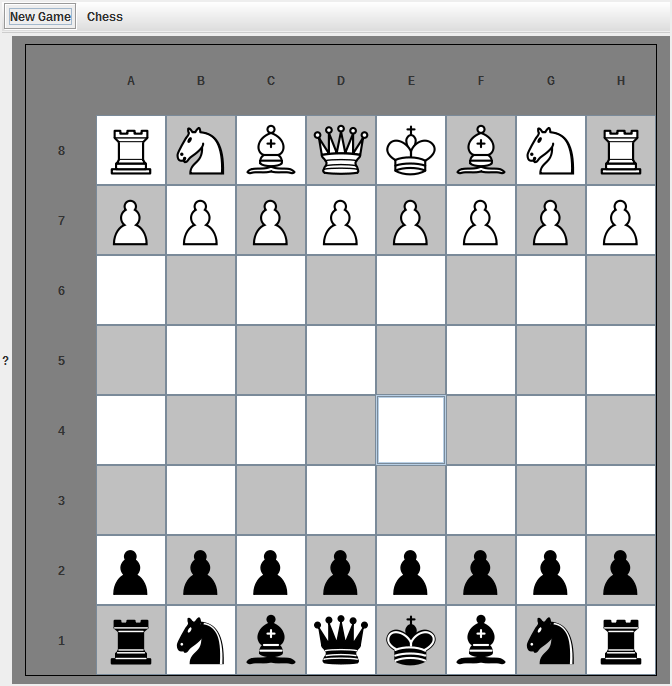
\includegraphics[scale=0.4]{ChessGUI.png}
  \caption{Start of Game Screenshot}
\end{figure}

\centerline{\textbf{Test Checklist}}
\begin{enumerate}
\item
  Create a Dropdown to choose between playing a classic game or playing a
  game with the new pieces already on the board, or available only
  by promotion. In the latter case, check whether the pieces will be able
  to be selected and visible upon the promotion of a pawn.
\item
  Make sure the coordinates of the board in the GUI
  correctly map to pieces in the internal board.
\end{enumerate}

\end{document}